手工课上老师给每位同学发了一张边长是$8$厘米的正方形彩纸.小王用剪刀从中剪下一个最大的圆(如图$1$),而小张先将彩纸折成$4$个小正方形,然后再从每个小正方形
中各剪下一个最大的圆(如图$2$),他俩都觉得自己的裁剪方式对彩纸的利用率比对方
高,请你帮忙算一下,给他俩评评理.($\text{利用率}=\frac{\text{剪下圆的面积总和}}{\text{彩纸面积}}\times100\%$)

\begin{center}
    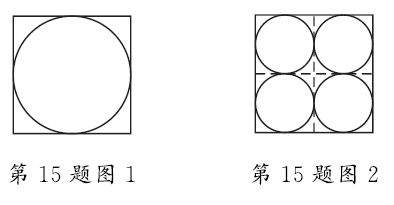
\includegraphics[height=4cm]{lib/image/MJA04030115.png}
\end{center}